%%%%%%%%%%%%%%%%%%%%%%%%%%%%%%%%%%%%%%%%%
% Short Sectioned Assignment LaTeX Template Version 1.0 (5/5/12)
% This template has been downloaded from: http://www.LaTeXTemplates.com
% Original author:  Frits Wenneker (http://www.howtotex.com)
% License: CC BY-NC-SA 3.0 (http://creativecommons.org/licenses/by-nc-sa/3.0/)
%%%%%%%%%%%%%%%%%%%%%%%%%%%%%%%%%%%%%%%%%

%----------------------------------------------------------------------------------------
%	PACKAGES AND OTHER DOCUMENT CONFIGURATIONS
%----------------------------------------------------------------------------------------

\documentclass[paper=a4, fontsize=11pt]{scrartcl} % A4 paper and 11pt font size

% ---- Entrada y salida de texto -----

\usepackage[T1]{fontenc} % Use 8-bit encoding that has 256 glyphs
\usepackage[utf8]{inputenc}
%\usepackage{fourier} % Use the Adobe Utopia font for the document - comment this line to return to the LaTeX default

% ---- Idioma --------

\usepackage[spanish, es-tabla]{babel} % Selecciona el español para palabras introducidas automáticamente, p.ej. "septiembre" en la fecha y especifica que se use la palabra Tabla en vez de Cuadro

% ---- Otros paquetes ----

\usepackage{url} % ,href} %para incluir URLs e hipervínculos dentro del texto (aunque hay que instalar href)
\usepackage{amsmath,amsfonts,amsthm} % Math packages
%\usepackage{graphics,graphicx, floatrow} %para incluir imágenes y notas en las imágenes
\usepackage{graphics,graphicx, float} %para incluir imágenes y colocarlas

% Para hacer tablas comlejas
%\usepackage{multirow}
%\usepackage{threeparttable}

%\usepackage{sectsty} % Allows customizing section commands
%\allsectionsfont{\centering \normalfont\scshape} % Make all sections centered, the default font and small caps

\usepackage{fancyhdr} % Custom headers and footers
\pagestyle{fancyplain} % Makes all pages in the document conform to the custom headers and footers
\usepackage{eurosym} % Para poder añadir el símbolo del euro
\fancyhead{} % No page header - if you want one, create it in the same way as the footers below
\fancyfoot[L]{} % Empty left footer
\fancyfoot[C]{} % Empty center footer
\fancyfoot[R]{\thepage} % Page numbering for right footer
\renewcommand{\headrulewidth}{0pt} % Remove header underlines
\renewcommand{\footrulewidth}{0pt} % Remove footer underlines
\setlength{\headheight}{13.6pt} % Customize the height of the header

\numberwithin{equation}{section} % Number equations within sections (i.e. 1.1, 1.2, 2.1, 2.2 instead of 1, 2, 3, 4)
%\numberwithin{figure}{section} % Number figures within sections (i.e. 1.1, 1.2, 2.1, 2.2 instead of 1, 2, 3, 4)
%\numberwithin{table}{section} % Number tables within sections (i.e. 1.1, 1.2, 2.1, 2.2 instead of 1, 2, 3, 4)

\setlength\parindent{0pt} % Removes all indentation from paragraphs - comment this line for an assignment with lots of text

\newcommand{\horrule}[1]{\rule{\linewidth}{#1}} % Create horizontal rule command with 1 argument of height

% Margins
\usepackage[margin=1.25in]{geometry}

% Begin section numbering at 0
\setcounter{section}{-1} 

% Hyperlinks
\usepackage{hyperref, xcolor}
\hypersetup{
  % hidelinks = true,   % Oculta todos los enlaces.
  colorlinks = true,   % Muestra todos los enlaces, sin bordes alrededor.
  linkcolor={black},     % Color de enlaces genéricos
  citecolor={black},   % Color de enlaces de referencias
  urlcolor={magenta}     % Color de enlaces de URL
}
  % Configuración del documento

%----------------------------------------------------------------------------------------
%	TÍTULO Y DATOS DE LOS ALUMNOS
%----------------------------------------------------------------------------------------

\title{	
	\normalfont \normalsize 
	\textsc{\textbf{Fundamentos de Redes (2017-2018)} \\ Doble Grado en Ingeniería Informática y Matemáticas \\ Universidad de Granada} \\ [25pt] 
	\horrule{0.5pt} \\[0.4cm]
	\huge Definición e implementación de un \\ protocolo de aplicación \\ 
	\horrule{2pt} \\[0.5cm] 
}

\author{Simón López Vico \\ Ana María Peña Arnedo \\ Alberto Jesús Durán López} 
\date{\normalsize\today}

%----------------------------------------------------------------------------------------
% DOCUMENTOg
%----------------------------------------------------------------------------------------

\begin{document}
	\maketitle       % título
	\newpage 
	\tableofcontents % índice
	\newpage
	
	

	
	
\section{Descripción de la aplicación, funcionalidad y actores que intervienen}
	
	
Esta práctica consiste en la implementación de un protocolo de aplicación que consta
de un servidor y dos clientes. El juego se basa en el famoso "Pilla-Pilla"   donde 
un jugador 'X' tendrá que alcanzar a otro 'Y'. Para ello, ambos se conectarán con un nombre de usuario correcto almacenado en el servidor. Por tanto, los movimientos que ambos hagan se enviarán a través del servidor hacia el otro cliente.
		
	
	
	
\section{Diagrama de estados del servidor}

\begin{figure}[h]
	\centering
	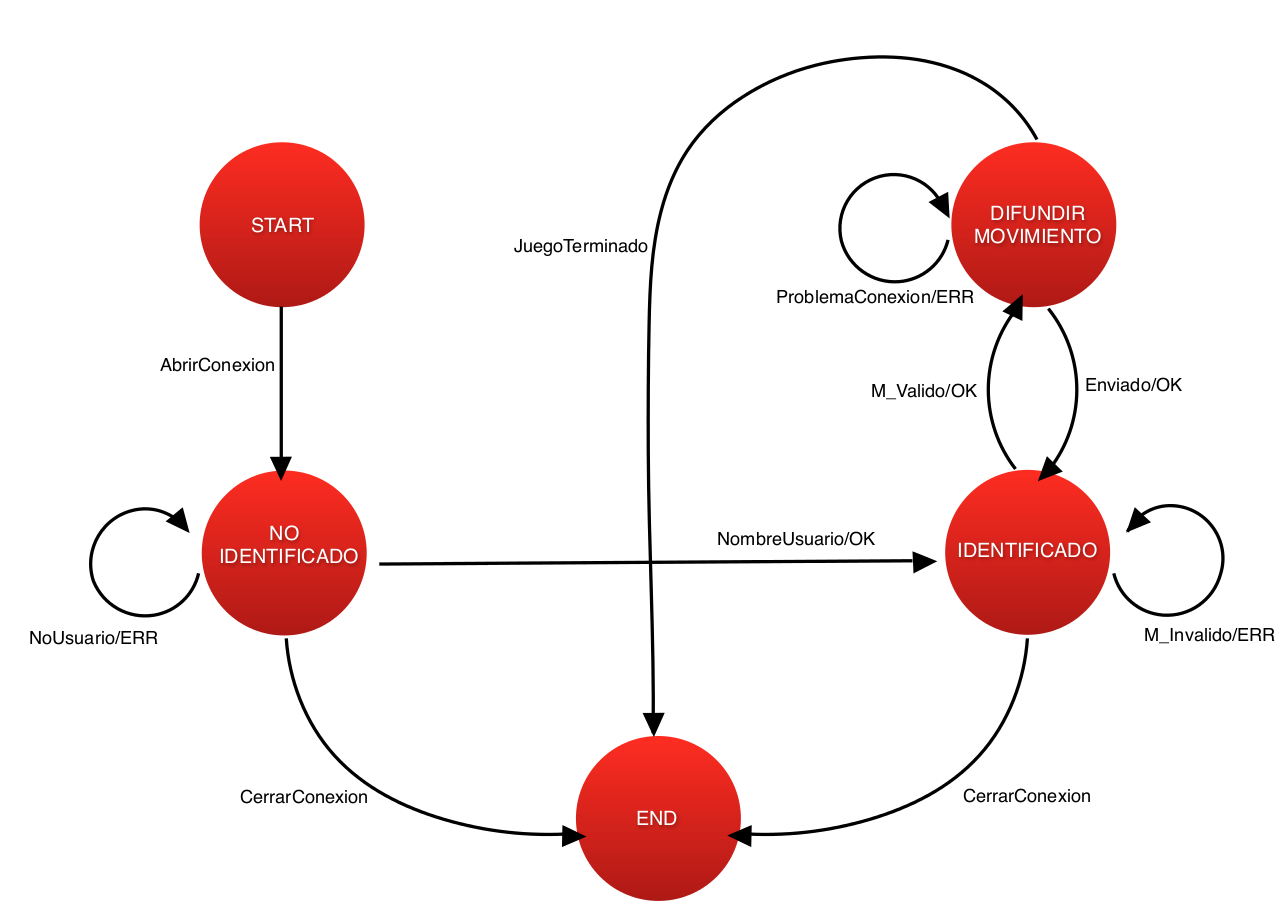
\includegraphics[width=.8\textwidth]{img/1}
	\caption{Diagrama de estados del servidor}
\end{figure}
	

Empezamos en el estado \textit{START}. El cliente abre la conexión hacia el servidor. Por tanto, pasará al estado \textit{IDENTIFICADO} si introduce un usuario correcto ó se quedará en el estado \textit{NO IDENTIFICADO} hasta que se autentifique correctamente. Una vez conectados ambos clientes, podrán realizar movimientos y pasar al estado \textit{DIFUNDIR MOVIMIENTO} un número indefinido de veces o pasar al estado \textit{END} si el juego se ha acabado. Cabe destacar que cada estado posee su propia comprobación de errores. \\

Para esta aplicación usamos \textit{sockets TCP} ya que nos ofrecen un servicio de transmisión orientado a conexión en el que se garantiza que los datos llegan en el orden en el que fueron enviados, sin errores ni repetición, de manera que nos proporciona control de flujo extremo a extremo y control de errores de forma transparente
	












\newpage

\section{Mensajes que intervienen}

\subsection{Tabla de estados del servidor}

\begin{figure}[h]
	\centering
	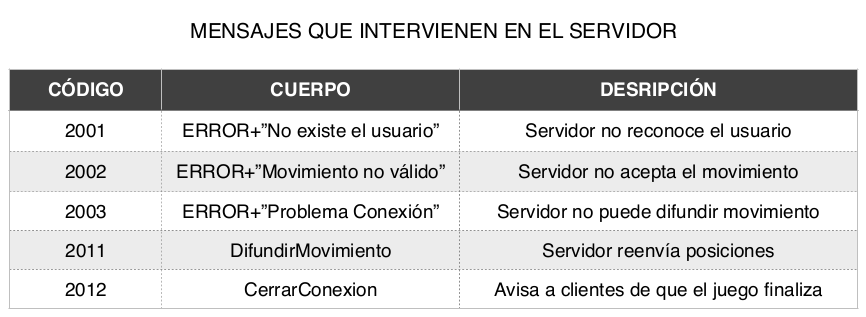
\includegraphics[width=.9\textwidth]{img/3}
	\caption{Mensajes que intervienen en el servidor}
\end{figure}







\subsection{Tabla de estados del cliente}	

\begin{figure}[h]
	\centering
	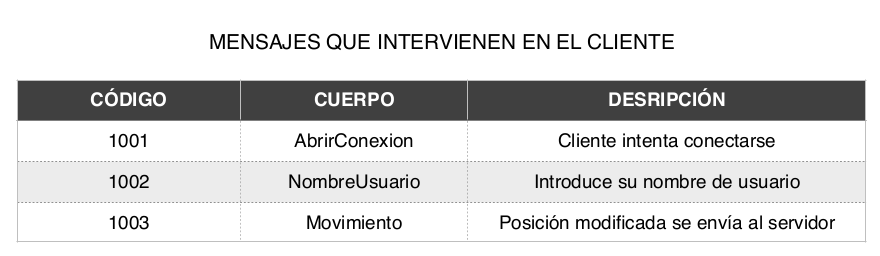
\includegraphics[width=.9\textwidth]{img/2}
	\caption{Mensajes que intervienen en el cliente}
\end{figure}


\newpage

\section{Descripción del programa}	

\subsection{Servidor}

La clase servidor contendrá las posiciones de cada uno de los jugadores y los semáforos necesarios para garantizar la exclusión mutua, así como los nombres de usuario admitidos por el servidor. En el constructor del servidor se asignará una posición aleatoria a cada uno de los jugadores. 

Esta clase estará compuesta por dos subclases, servidor uno y servidor dos, que heredan de la clase thread. Cada una de estas subclases contendrá un método ‘run’ similar. En dicho método el servidor estará esperando a que el cliente envíe su nombre de usuario. Tras recibirlo, comprobará que es correcto comparándolo con una lista de nombres aceptados por el servidor. Si no lo está, el servidor seguirá esperando hasta que el cliente envíe un nombre de usuario válido.

Si el nombre de usuario ya es válido, el servidor enviará la letra que corresponde a cada cliente, de manera que al primer cliente que se conecta se le asigna el carácter ‘X’ y al otro cliente se le asigna el carácter ‘O’. Después, imprimirá por pantalla que el cliente se ha conectado al servidor e inmediatamente después le enviará su posición en el mapa. 

A continuación, el servidor entrará en un bucle en el que comprobará, en cada iteración, que la distancia entre ambos jugadores es menor que la raíz de 2, es decir, que un jugador se encuentra en el 8-entorno del otro. Dentro de dicho bucle el servidor estará esperando a que el cliente le envíe su posición. Al recibirla, actualizará la variable que contiene la posición de dicho jugador y enviará a este cliente la posición del otro jugador.

Cuando el servidor salga de este bucle, enviará al cliente el mensaje ‘FIN’, lo que será interpretado por el cliente como que ha terminado el juego. Se imprimirá por pantalla el mensaje de que el cliente se ha desconectado y se cerrará el socket servicio.


\subsection{Cliente}
La clase cliente contendrá las posiciones del jugador controlado por el cliente en cuestión, así como las posiciones del contrincante. Al igual que en el servidor, en esta clase tendremos semáforos que garantizan la exclusión mutua, así como una hebra para conectarnos con el servidor. En el constructor del cliente se inicializarán cada uno de los semáforos y la hebra, y se lanzará para que empiece a ejecutarse. 

El cliente contendrá una subclase que hereda de la clase thread. Dicha clase contendrá el nombre de usuario del jugador, y el método ‘run’ para lanzar la hebra.

El programa cliente se ejecutará acompañado de un argumento que constituirá el nombre de usuario correspondiente al cliente que desea conectarse al servidor. Una vez ejecutado, se enviará al servidor dicho nombre. El servidor, como hemos comentado, le responderá o bien con el mensaje \textit{FAILED}  o bien con el carácter correspondiente asignado al jugador. Si el mensaje es \textit{FAILED}, se aborta el programa.

Al recibir el carácter correspondiente al jugador, se podría la posición asignada por el servidor al cliente. Seguidamente se imprimirá por pantalla el mapa incluyendo el símbolo del jugador en una determinada posición. En este momento, comienza el juego.

Se realizará un bucle del que se saldrá cuando el mensaje recibido desde el servidor sea \textit{FIN}. En este bucle, se introducirá un carácter para efectuar un movimiento. Inmediatamente después, se enviará la nueva posición del jugador al servidor, y el cliente le pedirá al servidor la posición de su adversario. 

Finalmente, al salir del bucle se imprimirá por pantalla \textit{FIN DEL JUEGO} y se cerrará el socket de servicio.

\newpage

\section{Evaluación de la aplicación}


\begin{figure}[h]
	\centering
	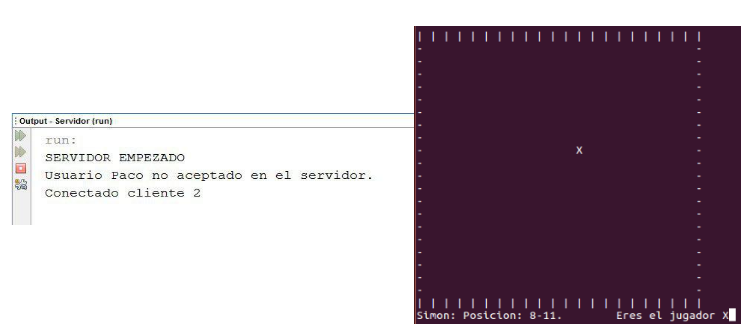
\includegraphics[width=1.1\textwidth]{img/erroneo}
	\caption{Autenticación errónea y correcta (asignación de letra)}
\end{figure}

	
\begin{figure}[h]
	\centering
	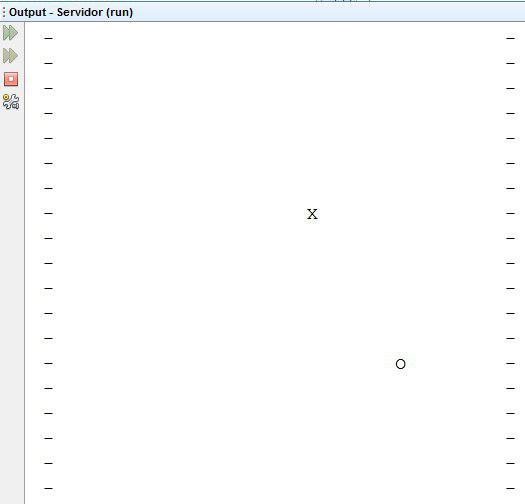
\includegraphics[width=.5\textwidth]{img/8}
	\caption{Vista del servidor cuando se conectan los dos clientes}
\end{figure}

\begin{figure}[h]
	\centering
	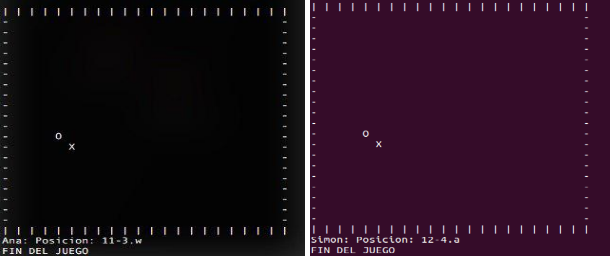
\includegraphics[width=1\textwidth]{img/esta}
	\caption{Fin del juego para ambos clientes}
\end{figure}





\newpage


\begin{figure}[h]
	\centering
	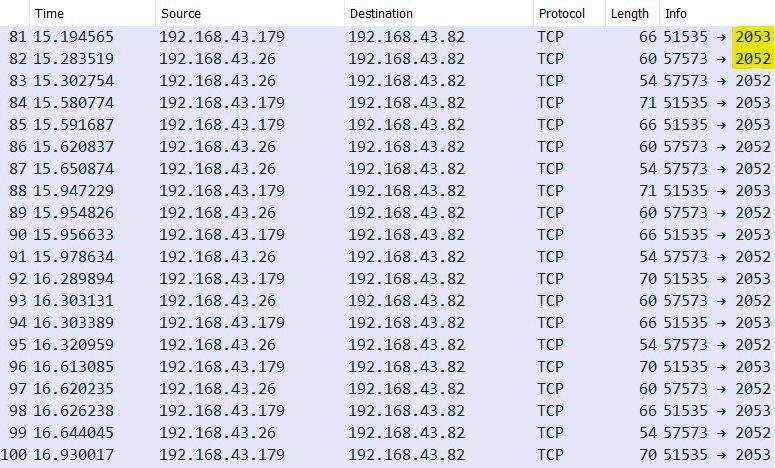
\includegraphics[width=.9\textwidth]{img/7}
	\caption{Captura de Wireshark. Comunicación a través de los puertos 2052 y 2053}
\end{figure}

\newpage

\section{Observaciones}



\end{document}